\documentclass[convert={outfile=\jobname.png}]{standalone}
\usepackage{base}
\usepackage{draw}
\usepackage{code}

\begin{document}

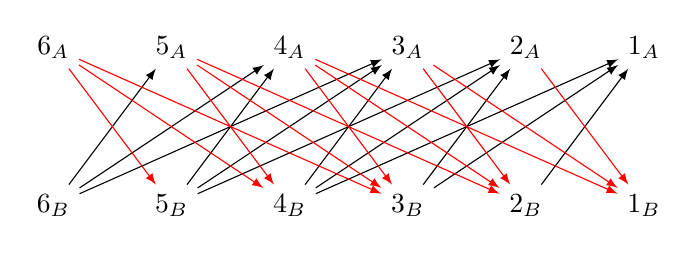
\begin{tikzpicture}
\node (01) at (-1.5*1, 0) {$1_B$};
\node (11) at (-1.5*1, 2) {$1_A$};
\node (02) at (-1.5*2, 0) {$2_B$};
\node (12) at (-1.5*2, 2) {$2_A$};
\node (03) at (-1.5*3, 0) {$3_B$};
\node (13) at (-1.5*3, 2) {$3_A$};
\node (04) at (-1.5*4, 0) {$4_B$};
\node (14) at (-1.5*4, 2) {$4_A$};
\node (05) at (-1.5*5, 0) {$5_B$};
\node (15) at (-1.5*5, 2) {$5_A$};
\node (06) at (-1.5*6, 0) {$6_B$};
\node (16) at (-1.5*6, 2) {$6_A$};
\draw[->, >=latex, color=black] (02) to (11);
\draw[->, >=latex, color=black] (03) to (12);
\draw[->, >=latex, color=black] (04) to (13);
\draw[->, >=latex, color=black] (05) to (14);
\draw[->, >=latex, color=black] (06) to (15);
\draw[->, >=latex, color=black] (03) to (11);
\draw[->, >=latex, color=black] (04) to (12);
\draw[->, >=latex, color=black] (05) to (13);
\draw[->, >=latex, color=black] (06) to (14);
\draw[->, >=latex, color=black] (04) to (11);
\draw[->, >=latex, color=black] (05) to (12);
\draw[->, >=latex, color=black] (06) to (13);
\draw[->, >=latex, color=red] (12) to (01);
\draw[->, >=latex, color=red] (13) to (02);
\draw[->, >=latex, color=red] (14) to (03);
\draw[->, >=latex, color=red] (15) to (04);
\draw[->, >=latex, color=red] (16) to (05);
\draw[->, >=latex, color=red] (13) to (01);
\draw[->, >=latex, color=red] (14) to (02);
\draw[->, >=latex, color=red] (15) to (03);
\draw[->, >=latex, color=red] (16) to (04);
\draw[->, >=latex, color=red] (14) to (01);
\draw[->, >=latex, color=red] (15) to (02);
\draw[->, >=latex, color=red] (16) to (03);
\end{tikzpicture}

\end{document}